\documentclass[letterpaper,10pt]{article}
\usepackage[utf8]{inputenc}
\usepackage{amsmath}
\usepackage{tikz}

\title{A bit about floating point representations: \\ Reals, Bitvectors, Ordinals, and Ulps}
\author{Bill Zorn}

\begin{document}

\maketitle

\begin{abstract}
 Floating point number representations are complicated; we seek to provide a crisp definition of the terms in the title and the relationships between them. Traditionally, floating point numbers are thought of as representing the values of real numbers. In some situations, we find that it makes more sense to impose an ordering on them and treat them like signed integer ordinals, for example when computing units in the last place difference (ulps), or the Posix \texttt{nextafter()} function. We formalize the mathematical underpinnings of these relationships as operations on bitvectors.
\end{abstract}

\section{Introduction}

Some things are difficult to get right, and floating point is one of those things. Sometimes the difference between $\frac{4}{3}$ and 1.3333334 is unimportant, but sometimes it is the difference between the right answer and the wrong answer, or between SAT and UNSAT. The problem is that while they represent familiar real numbers, floating point numbers are incredibly specific: if you really want the right answer, you have to be precise down to the last bit. And for most people, a vector of bits like \texttt{0b00111111101010101010101010101011} is much less intuitive to think about than the real (rational, even) number $\frac{4}{3}$.

The purpose of this text is to write down in a convient place, once and for all, the meaning of floating point numbers, and formalize the conversions between various bitvector representations that are compatible with the IEEE 754-2008 standard \cite{ieee754-2008} but general enough to be useful in other applications, for example when devising constraints for SMT solvers. This way, the author (and any other interested implementers) can avoid the trouble of having to write all this down again, or risk getting a bit of it wrong.

\section{Reals as Bitvectors}

A floating point number is a triple of three things: a sign $s$, an exponent $e$, and a significand $c$. $s$ is either 0 or 1 and $e$ is a positive or negative integer. We would like $c$ to represent a fractional value; to do this, we can make it a positive integer and keep around some notion of precision $p$ which records the number of digits in $c$, as represented in a base $b$. The real value represented by a number in this representation is given in Equation \ref{eq:real}.

\begin{align} \label{eq:real}
 (-1)^s \times b^e \times (c \times b^{1 - p})
\end{align}

For lack of another widely supported alternative, we will specialize our discussion here to the IEEE 754 (binary) standard. We fix $b = 2$, and commit to representing $c$ as a bitvector $C$ of size $p$. As we can see in Equation \ref{eq:real2}, this eliminates all terms not explicit in our triple, assuming we can take the size of a bitvector and perform arithmetic on it as an unsigned integer.

\begin{align} \label{eq:real2}
 (-1)^s \times 2^e \times (uint(C) \times 2^{1 - size(C)})
\end{align}

The IEEE 754 assigns some floating point numbers to represent values other than finite real numbers. Specifically, numbers with greater than some ``maximum'' $e$ and $c = 0$ represent infinite real numbers of the appropriate sign, and numbers with greater than this ``maximum'' $e$ but $c \neq 0$ represent something that is not a real number, or NaN, such as the indeterminate result of $\frac{0}{0}$. If we commit to representing $e$ as a bitvector $E$ of size $w$, then this ``maximum'' value is $emax = 2^{w-1} - 1$, the largest positive integer a bitvector of size $w$ can represent under a two's complement system. Instead of using two's complement directly, the IEEE 754 standard specifies a biased representation, defining also a minimum exponent $emin = 1 - emax$ and $e = max(uint(E) - emax, emin)$.

Since the values of $e$ and $c$ are already represented as bitvectors, we might as well put $s$ in a 1-bit vector $S$ with $s = uint(S)$. We fully specify the meaning of our mapping from triples of bitvectors to finite real numbers (or one of two infinite real numbers, or a symbol representing something other than a real number) in Equation \ref{eq:real3},

\begin{align} \label{eq:real3}
 real(S, E, C) =
 \begin{cases}
  NaN                                           & e > emax \land c \neq 0 \\
  (-1)^s \times \infty                          & e > emax \land c = 0    \\
  (-1)^s \times 2^e \times (c \times 2^{1 - p}) & e \leq emax
 \end{cases}
\end{align}
where:
\begin{description}
 \item $w = size(E)$
 \item $p = size(C)$
 \item $emax = 2^{w-1} - 1$
 \item $emin = 1 - emax$
 \item $s = uint(S)$
 \item $e = max(uint(E) - emax, emin)$
 \item $c = uint(C)$.
\end{description}

Let us call this the explicit triple of bitvectors or ``explicit triple'' representation of a floating point number. Except for its neglect of the distinction between quiet and signaling NaNs, this formulation agrees completely with IEEE 754, assuming the ability to identify the correct bitvectors $S$, $E$, and $C$. As presented in Equation \ref{eq:real3}, some real numbers can be represented in multiple ways. For example, the triple $(\texttt{0b0}, \texttt{0b01}, \texttt{0b10})$ represents $(-1)^0 \times 2^0 \times (2 \times 2^{-1}) = 1.0$. But so does $(\texttt{0b0}, \texttt{0b10}, \texttt{0b01})$, as $(-1)^0 \times 2^1 \times (1 \times 2^{-1}) = 1.0$ as well. Similarly, having $E$ as 0 or 1 gives an equivalent $e = emin$ due to the max in the definition of $e$. And there are $2 \times (2^w - 1)$ ways to represent 0.

To take advantage of these redundancies and eliminate a bit from the representation, the IEEE 754 standard represents the first bit of $C$ implicitly. Any real number representable with $e > emin$ and $C[0] = 0$ (i.e. the first bit of $C$ is 0, or $c < 2^{p-1}$) can be similarly represented by shifting $C$ 1 bit to the left and subtracting 1 from E (which has the effect of subtracting 1 from $e$ as well, given $e > emin$). Thus each representable number has a canonical representation, where either $C[0] = 1$, or $e = emin$. 

To take advantage of this, the IEEE 754 standard records the first bit of $C$ implicitly as the otherwise unused case where $E$ is 0, and keeps track of the rest of $C$ as a shorter bitvector $T$ of size $p - 1$. If $E$ is 0, the corresponding $C$ is $concat(\texttt{0b0}, T)$, otherwise $C$ is $concat(\texttt{0b1}, T)$. This ensures that all numbers are represented with their canonical representation: correctly converting a bitvector from the IEEE 754 binary interchange format to the explicit triple representation of Equation \ref{eq:real3} will always yield a canonical result. The only real number with multiple canonical representations is 0, which can take either sign.

Equation \ref{eq:real4a} defines conversion between formats; in combination with Equation \ref{eq:real3}, it is sufficient to fully specify the mapping from bitvectors in the IEEE 754 binary interchange formats to real numbers (or NaN), assuming the fields $S$, $E$, and $T$ are available or can be correctly extracted from a concatenated binary interchange bitvector (such as a fimiliar 32-bit \texttt{float}). Going the other way is trivial, as we can always recover $T$ from $C$ by dropping the first bit, as in Equation \ref{eq:real4b}.

\begin{align} 
 C &= \label{eq:real4a}
 \begin{cases}
  concat(\texttt{0b0}, T) & uint(E) = 0 \\
  concat(\texttt{0b1}, T) & uint(E) \neq 0
 \end{cases} \\
 T &= extract(p-2, 0, C)  \label{eq:real4b}
\end{align}

The explicit mapping from IEEE 754 bitvectors to reals is given in Equation \ref{eq:real5},

\begin{align} \label{eq:real5}
 real(S, E, T) =
 \begin{cases}
  NaN                                                      & e > emax \land c \neq 0 \\
  (-1)^s \times \infty                                     & e > emax \land c = 0    \\
  (-1)^s \times 2^e \times ((c' + 2^{p-1}) \times 2^{1-p}) & emin < e \leq emax      \\
  (-1)^s \times 2^e \times (c' \times 2^{1 - p})           & e = emin
 \end{cases}
\end{align}
where:
\begin{description}
 \item $w = size(E)$
 \item $p = size(T) + 1$
 \item $emax = 2^{w-1} - 1$
 \item $emin = 1 - emax$
 \item $s = uint(S)$
 \item $e = max(uint(E) - emax, emin)$
 \item $c' = uint(T)$.
\end{description}

Let us call this the implicit triple of bitvectors, or ``implicit triple'' or ``IEEE 754 triple'' representation of floating point numbers. We also say that the IEEE binary interchange format uses a ``packed bitvector'' or ``implicit packed'' or just ``packed'' representation $B = concat(S, E, T)$. $S$ can always be recovered, and $E$ and $T$ can be recovered as long as $w$ or $p$ is known. 

This formulation is equivalent to the description in section 3.4 of \cite{ieee754-2008}. For clarity, we have tried to name our terms according to similar concepts from the IEEE 754 standard, finally running into problems with the incomparable $c'$. The treatment here should not differ materially from the IEEE 754 standard, and is intended mostly to provide Equations \ref{eq:real3} and \ref{eq:real5} and their requisite definitions in a compact form for implementers of bitvector programs.

It should be noted that most hardware implementations use the packed bitvector representation; i.e. on a typical implementation using 32-bit single-precision floats, $\frac{4}{3}$ would be represented as 
\begin{align*}
 \texttt{0b00111111101010101010101010101011} \text{,}
\end{align*}
which would unpack (assuming $w=8$, $p=24$) to the implicit triple 
\begin{align*}
 (\texttt{0b0}, \texttt{0b01111111}, \texttt{0b01010101010101010101011})
\end{align*}
or the explicit triple 
\begin{align*}
 (\texttt{0b0}, \texttt{0b01111111}, \texttt{0b101010101010101010101011}) \text{.}
\end{align*}
The floating point theory defined as part of the SMT-LIB standard specifies floating point literals in a form equivalent to the implicit triple representation, i.e. the term of sort \texttt{(\_ FloatingPoint 8 24)}, where 8 and 24 are $w$ and $p$ respectively, that represents the real number closest to $\frac{4}{3}$, is written 
\begin{align*}
 \texttt{(fp \#b0 \#b01111111 \#b01010101010101010101011)} \text{.}
\end{align*}
\section{Reals as Bitvectors as Ordinals}

Floating point numbers represent real numbers, but since they do so with bitvectors, they have some properties that bear more resemblance to integers. For example, it might be more important to know how close two real values $r1$ and $r2$ are, not in terms of their real difference $r2 - r1$, but in terms of the number of representable floating point numbers that exist between them. This quantity, ulps, is entirely dependent on the properties of the floating point representation in question and independent of the properties of real numbers.

To compute ulps, it can be helpful to think of floating point numbers as ordinals. By ``ordinals,'' we mean signed integers that impose a total ordering on all real values representable with a given floating point representation, not true ordinal numbers in the mathematical sense. A similar notion is presented in the IEEE 754 standard's totalOrder predicate. The floating point numbers of a given representation with finite $w$ and $p$ form a finite set, so a total ordering is possible, and indeed that is what totalOrder provides. However that ordering has some properties that might be surprising: all of the NaNs are ordered, which is necessary for a total ordering but perhaps not helpful, and more problematically -0.0 is less than +0.0, even though both have the same real value.

Several different orderings are possible: we choose one that is hopefully the least surprising for implementers, and discuss how it compares to the totalOrder predicate and other alternatives. We implement this ordering with a function $ord(F)$, which takes a floating point number $F$ in some known representation (such as a packed bitvector or implicit triple with $w$ and $p$ known) and produces a positive or negative integer. We would like $ord(F)$ to have the following properties:

\begin{enumerate}
 \item If $real(F) = 0.0$, $ord(F) = 0$. I.e. all floating point numbers that represent a real value of zero (including ones that have a negative sign) have an order of 0.
 \item If $real(F_1) = real(F_2)$, then $ord(F_1) = ord(F_2)$. I.e. floating point numbers that represent the same real value have the same order.
 \item If $real(F_1) < real(F_2)$, then $ord(F_1) < ord(F_2)$. I.e. floating point numbers are ordered by their real value.
 \item If $real(F_1) = -\infty$ and $real(F_2) = \infty$, then $ord(F_2) - ord(F_1)$ is equal to the number of distinct real values the representation can represent (including the two infinities, but not including any NaNs) minus one. I.e. the ordinals are tightly packed: there is no positive $i$ such that there is no $F$ that has $ord(F)$ and yet there is some $F'$ that has $ord(F') > i$, or analogously for negative $i$.
 \item If $real(F)$ is NaN, then $ord(F)$ is undefined. In general, the order of a floating point number that represents NaN cannot be relied upon to be meaningful, so the safest thing to do is refuse to assign it meaning. An implementation might want to do something in this case like return an error, or extend the notion of an ordinal to include NaN and return that. In some cases there might be implementation-specific meaning, which we will discuss in more detail.
\end{enumerate}


\begin{figure}[h!]
 \centering
 \caption{Floating point numbers with $w=2$, $p=2$} \label{fig:numberline1}
 \smallskip
 \resizebox{\textwidth}{!}{
 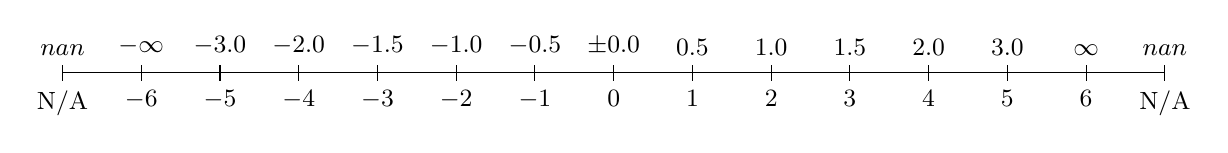
\begin{tikzpicture}[scale=1.0]
  \draw (-7,0) -- (7,0);
   \foreach \i/\o/\r in {0/0/\pm0.0,1/1/0.5,2/2/1.0,3/3/1.5,4/4/2.0,5/5/3.0,6/6/\infty,7/\text{N/A}/nan,-1/-1/-0.5,-2/-2/-1.0,-3/-3/-1.5,-4/-4/-2.0,-5/-5/-3.0,-6/-6/-\infty,-7/\text{N/A}/nan}
   {
    \draw (\i,0.1) -- + (0,-0.2) node[below] {\small $\o$} + (0,0.0) node[above] {\small $\r$};
   }
    \end{tikzpicture}
 }
\end{figure}

\begin{figure}[h!]
 \centering
 \caption{Floating point numbers with $w=2$, $p=2$, distributed by real value} \label{fig:numberline2}
 \smallskip
 \centering
 \resizebox{\textwidth}{!}{
 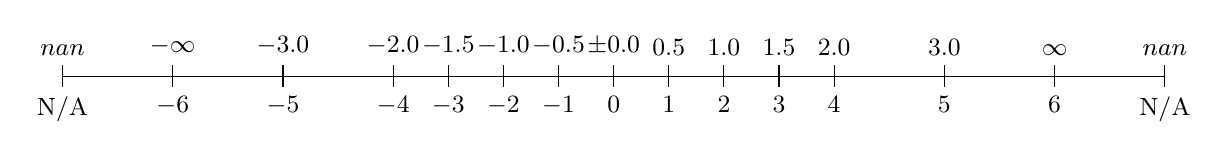
\begin{tikzpicture}[scale= 7.0/5.0]
  \draw (-5,0) -- (5,0);
   \foreach \i/\o/\r in {0.0/0/\pm0.0,0.5/1/0.5,1.0/2/1.0,1.5/3/1.5,2.0/4/2.0,3.0/5/3.0,4.0/6/\infty,5.0/\text{N/A}/nan,-0.5/-1/-0.5,-1.0/-2/-1.0,-1.5/-3/-1.5,-2.0/-4/-2.0,-3.0/-5/-3.0,-4.0/-6/-\infty,-5.0/\text{N/A}/nan}
   {
    \draw (\i,0.1) -- + (0,-0.2) node[below] {\small $\o$} + (0,0.0) node[above] {\small $\r$};
   }
    \end{tikzpicture}
 }
\end{figure}

\bibliographystyle{ieeetr}
\bibliography{ref}

\end{document}
